\section{Software Architecture}
\label{sec:architecture}

\subsection{Dependency Layering}

IsalSR enforces strict dependency isolation:

\begin{verbatim}
experiments/, benchmarks/  -> anything (numpy, scipy, matplotlib, ...)
isalsr.search              -> numpy
isalsr.evaluation          -> numpy, scipy
isalsr.adapters            -> optional: networkx, sympy
isalsr.core                -> ZERO external dependencies (stdlib only)
\end{verbatim}

The core layer (\texttt{isalsr.core}) has zero external dependencies,
enabling lightweight distribution and reproducibility.

\begin{figure}[h]
\centering
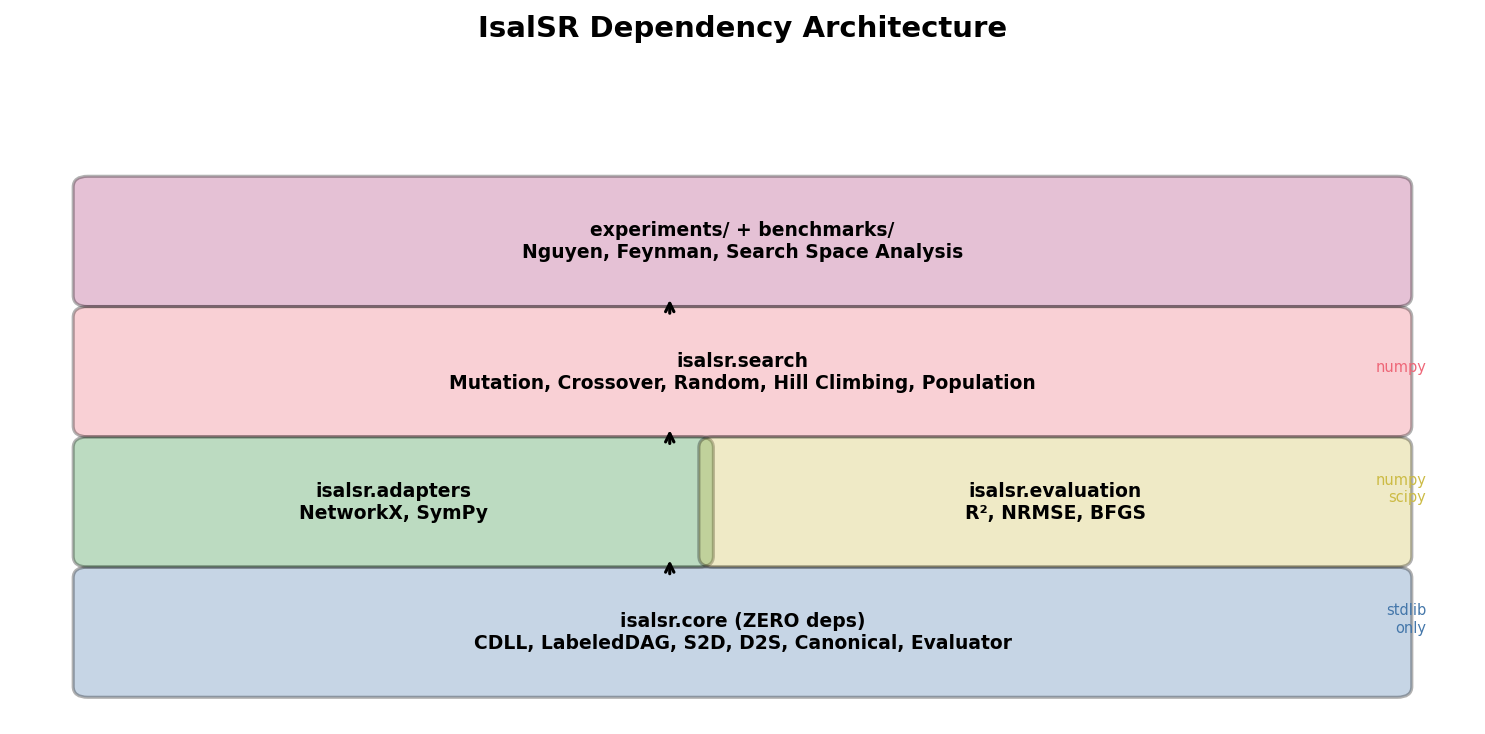
\includegraphics[width=\textwidth]{figures/architecture.png}
\caption{IsalSR dependency architecture. Each layer only depends on layers
below it. The core layer has zero external dependencies.}
\label{fig:architecture}
\end{figure}

\subsection{Module Inventory}

\begin{table}[h]
\centering
\caption{IsalSR module inventory with line counts and purposes.}
\label{tab:modules}
\begin{tabular}{lrl}
\toprule
Module & Lines & Purpose \\
\midrule
\texttt{core/cdll.py} & 130 & Circular doubly linked list (from IsalGraph) \\
\texttt{core/labeled\_dag.py} & 480 & LabeledDAG with cycle detection \\
\texttt{core/node\_types.py} & 140 & NodeType enum, arity registry \\
\texttt{core/string\_to\_dag.py} & 240 & S2D decoder (tokenizer + executor) \\
\texttt{core/dag\_to\_string.py} & 310 & D2S greedy encoder \\
\texttt{core/canonical.py} & 350 & Canonical string (exhaustive + pruned) \\
\texttt{core/dag\_evaluator.py} & 200 & Numerical evaluation (protected ops) \\
\texttt{core/algorithms/} & 110 & D2S algorithm variants (4 strategies) \\
\midrule
\texttt{adapters/} & 250 & NetworkX, SymPy bridges \\
\texttt{evaluation/} & 200 & Fitness metrics, BFGS constant optimizer \\
\texttt{search/} & 380 & Token-aware operators, search algorithms \\
\midrule
\textbf{Total source} & \textbf{$\sim$2800} & \\
\textbf{Total tests} & \textbf{286} & Unit + integration + property \\
\bottomrule
\end{tabular}
\end{table}

\subsection{Testing Strategy}

The project follows a rigorous multi-layer testing strategy:
\begin{itemize}[nosep]
  \item \textbf{Unit tests} (252): Core data structures, algorithms, operators.
    No external dependencies required.
  \item \textbf{Integration tests} (26): NetworkX/SymPy adapter round-trips,
    fitness metrics, BFGS constant optimization.
  \item \textbf{Property tests} (8): Hypothesis-based generative tests for
    round-trip, DAG acyclicity, canonical idempotency, evaluation finiteness.
\end{itemize}

All 286 tests pass with \texttt{ruff check} (linting) and
\texttt{mypy --strict} (type checking) clean.

\subsection{Proposal Alignment Guard}

A custom Claude Code agent (\texttt{proposal-guard}) validates every
implementation phase against the advisor's constraints:
\begin{enumerate}[nosep]
  \item No novel SR method is implemented.
  \item Every string modification is followed by canonicalization.
  \item The $O(k!)$ reduction is the main claim.
  \item Benchmarks use standard datasets.
\end{enumerate}
Across 7 phases, 78/80 alignment checks passed (2 non-blocking warnings).
